% ===========================================================================
% manuscript.tex — the ORCHESTRATOR. It owns the preamble and the \input order
% of the paper; it holds no prose itself, and compiles to manuscript.pdf. This
% whole folder (renders/manuscript/) is the unit you sync to Overleaf.
%
% Two kinds of inputs, two owners:
%
%   sections/*.tex      PROSE, no data. HAND-WRITTEN — live-edit on Overleaf.
%
%   generated/*.tex     GENERATED from the data by reports/manuscript/*.qmd
%   generated/figures/  (the methods & results sections, the model table, the
%   generated/tabs/     figures, and a copy of the bibliography). NEVER hand-edit
%   generated/*.bib     these — re-render and they refresh:
%                           quarto render reports/manuscript
% ===========================================================================
\documentclass[11pt]{article}

\usepackage[a4paper, margin=1in]{geometry}
\usepackage[utf8]{inputenc}
\usepackage{graphicx}
\usepackage{natbib}
\usepackage{booktabs}
\usepackage{hyperref}

\title{Framing effects on consumer purchase intention: \\
       a mediation and moderation analysis}
\author{Your Name}
\date{\today}

\begin{document}
\maketitle

\begin{abstract}
% sections/abstract.tex — PROSE (no data). Hand-written; live-edit on Overleaf.
We test whether messaging frames (scarcity, sustainability, social proof, and a
combined frame) increase purchase intention for everyday consumer products,
whether this effect is mediated by perceived value, and whether it is moderated
by price sensitivity. Data, code, and outputs all live in the same git
repository as this manuscript.

\end{abstract}

% ---- Prose (hand-written, Overleaf-owned) ---------------------------------
% sections/introduction.tex — PROSE (no data). Hand-written; live-edit on Overleaf.
\section{Introduction}

Mediation and moderation logic follows the classical framework
\citep{baron1986} and the regression-based approach in \citet{hayes2017}.


% ---- Generated from reports/manuscript/*.qmd (do not hand-edit) -----------
% GENERATED FROM reports/manuscript/methods.qmd — DO NOT EDIT BY HAND.
% Edit the prose in the .qmd, then: quarto render reports/manuscript

\section{Methods}

We analysed a simulated consumer decision-making dataset of 300
participants, each randomly assigned to one of 5 message-framing
conditions (a plain control plus scarcity, sustainability, social-proof,
and combined frames). After viewing the framed product, participants
reported multi-item measures of price sensitivity, sustainability
concern, brand trust, and perceived value, followed by their purchase
intention and a hypothetical buy decision.

Multi-item scales were averaged into composite scores after
reverse-scoring the relevant brand-trust item, and a value of \(-99\)
was treated as missing. Data were cleaned with scripted,
version-controlled steps; the full codebook and cleaning code live in
the project repository. All models were estimated in R with ordinary
least squares (\texttt{lm}). Every figure and table in this paper is
generated directly from the analysis code, so the reported numbers
cannot drift from the analysis.

% GENERATED FROM reports/manuscript/results.qmd — DO NOT EDIT BY HAND.
% Edit the prose in the .qmd, then: quarto render reports/manuscript

\section{Results}

\subsection{Main effect}

Relative to the control frame, the combined frame raised purchase
intention by 0.58 points on the seven-point scale (\(p = 0.008\)).
Figure\textasciitilde{}\ref{fig:main} shows the full pattern across
conditions.

\begin{figure}[h]
  \centering
  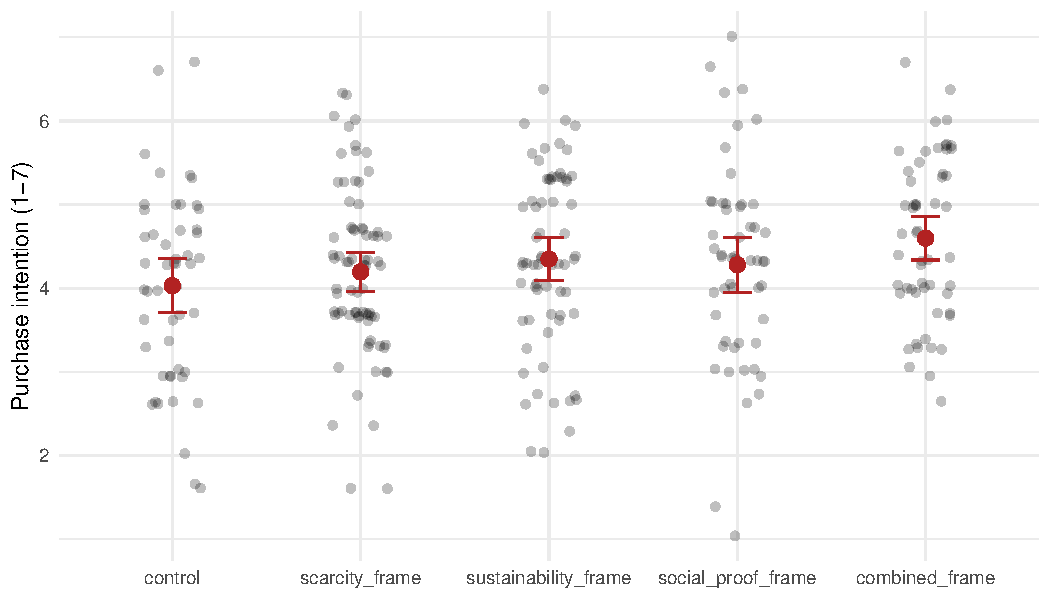
\includegraphics[width=0.85\textwidth]{generated/figures/fig_01_pi_by_condition.pdf}
  \caption{Purchase intention by condition. Red points are condition means with 95\% confidence intervals.}
  \label{fig:main}
\end{figure}

\subsection{Mediation through perceived value}

The frames also shifted perceived value upward, and perceived value
strongly predicted purchase intention
(Figure\textasciitilde{}\ref{fig:mediation}); adding it to the outcome
model attenuated the condition coefficients, the signature of an
indirect path.

\begin{figure}[h]
  \centering
  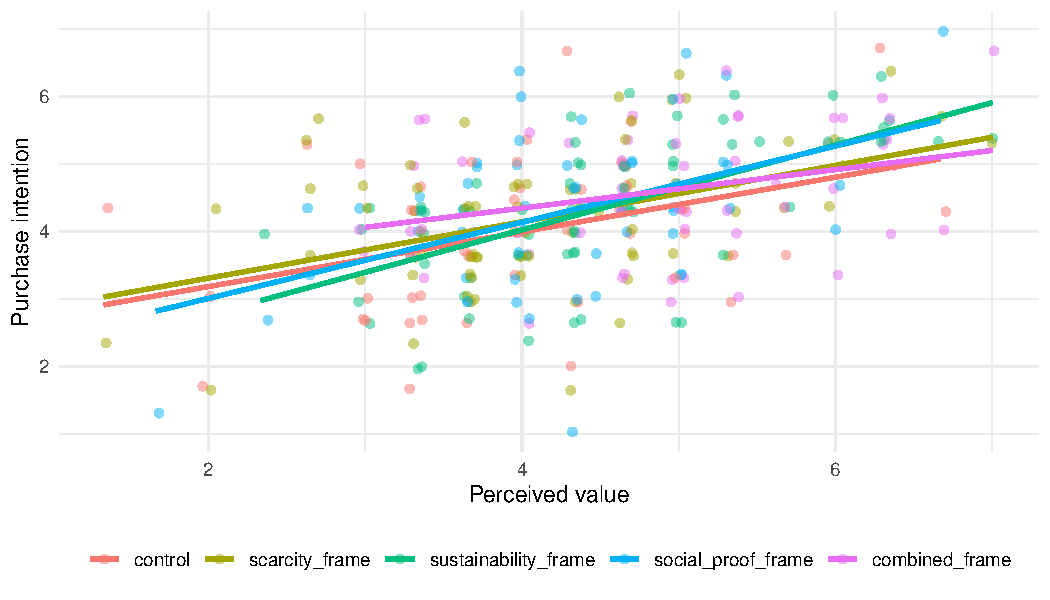
\includegraphics[width=0.85\textwidth]{generated/figures/fig_02_mediation_scatter.pdf}
  \caption{Perceived value predicts purchase intention; the frames shift perceived value upward, producing an indirect path.}
  \label{fig:mediation}
\end{figure}

\subsection{Moderation by price sensitivity}

The combined-frame boost was attenuated among the most price-sensitive
respondents (Figure\textasciitilde{}\ref{fig:moderation}).

\begin{figure}[h]
  \centering
  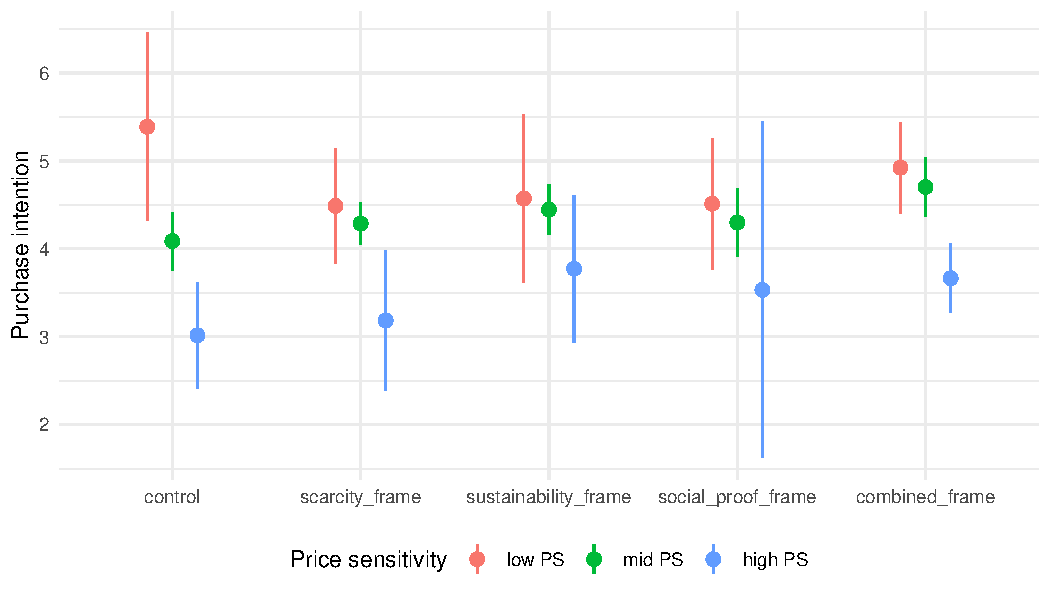
\includegraphics[width=0.85\textwidth]{generated/figures/fig_03_moderation.pdf}
  \caption{Condition $\times$ price sensitivity: the combined-frame boost shrinks for high-price-sensitive respondents.}
  \label{fig:moderation}
\end{figure}

\subsection{Model estimates}

Table\textasciitilde{}\ref{tab:models} collects the coefficients behind
the figures above. It is generated by
\texttt{reports/manuscript/results.qmd} and written into
\texttt{generated/tabs/}, so the paper's numbers track the analysis
exactly.

\begin{table}

\caption{\label{tab:models}Model estimates with 95\% confidence intervals.}
\centering
\begin{tabular}[t]{llrrrrr}
\toprule
Model & Term & Estimate & SE & CI low & CI high & p\\
\midrule
total & (Intercept) & 4.08 & 0.25 & 3.59 & 4.58 & 0.000\\
total & conditionscarcity\_frame & 0.14 & 0.20 & -0.26 & 0.54 & 0.494\\
total & conditionsustainability\_frame & 0.31 & 0.21 & -0.09 & 0.72 & 0.133\\
total & conditionsocial\_proof\_frame & 0.24 & 0.22 & -0.19 & 0.67 & 0.271\\
total & conditioncombined\_frame & 0.58 & 0.22 & 0.15 & 1.01 & 0.008\\
\addlinespace
total & age & 0.00 & 0.01 & -0.01 & 0.01 & 0.858\\
total & genderman & -0.03 & 0.14 & -0.30 & 0.24 & 0.816\\
total & gendernon\_binary & -0.46 & 0.34 & -1.14 & 0.21 & 0.175\\
total & genderprefer\_not\_to\_say & 0.12 & 0.30 & -0.46 & 0.71 & 0.676\\
total & income\_group.L & -0.18 & 0.13 & -0.43 & 0.08 & 0.177\\
\addlinespace
total & income\_group.Q & 0.02 & 0.10 & -0.18 & 0.23 & 0.841\\
mediator & (Intercept) & 4.06 & 0.24 & 3.58 & 4.55 & 0.000\\
mediator & conditionscarcity\_frame & 0.04 & 0.20 & -0.34 & 0.43 & 0.820\\
mediator & conditionsustainability\_frame & 0.48 & 0.20 & 0.09 & 0.87 & 0.016\\
mediator & conditionsocial\_proof\_frame & 0.20 & 0.21 & -0.22 & 0.61 & 0.351\\
\addlinespace
mediator & conditioncombined\_frame & 0.85 & 0.21 & 0.44 & 1.26 & 0.000\\
mediator & age & 0.00 & 0.01 & -0.01 & 0.01 & 0.877\\
mediator & genderman & -0.11 & 0.13 & -0.37 & 0.15 & 0.413\\
mediator & gendernon\_binary & -0.07 & 0.33 & -0.72 & 0.58 & 0.832\\
mediator & genderprefer\_not\_to\_say & 0.43 & 0.29 & -0.13 & 1.00 & 0.132\\
\addlinespace
mediator & income\_group.L & -0.10 & 0.12 & -0.35 & 0.15 & 0.424\\
mediator & income\_group.Q & 0.04 & 0.10 & -0.15 & 0.24 & 0.665\\
outcome\_w\_m & (Intercept) & 2.23 & 0.32 & 1.60 & 2.87 & 0.000\\
outcome\_w\_m & conditionscarcity\_frame & 0.12 & 0.18 & -0.24 & 0.48 & 0.516\\
outcome\_w\_m & conditionsustainability\_frame & 0.09 & 0.19 & -0.28 & 0.46 & 0.630\\
\addlinespace
outcome\_w\_m & conditionsocial\_proof\_frame & 0.15 & 0.20 & -0.24 & 0.54 & 0.443\\
outcome\_w\_m & conditioncombined\_frame & 0.19 & 0.20 & -0.20 & 0.59 & 0.334\\
outcome\_w\_m & perceived\_value & 0.46 & 0.06 & 0.35 & 0.57 & 0.000\\
outcome\_w\_m & age & 0.00 & 0.01 & -0.01 & 0.01 & 0.784\\
outcome\_w\_m & genderman & 0.02 & 0.12 & -0.22 & 0.26 & 0.888\\
\addlinespace
outcome\_w\_m & gendernon\_binary & -0.43 & 0.31 & -1.04 & 0.17 & 0.160\\
outcome\_w\_m & genderprefer\_not\_to\_say & -0.07 & 0.27 & -0.60 & 0.46 & 0.786\\
outcome\_w\_m & income\_group.L & -0.13 & 0.12 & -0.36 & 0.10 & 0.267\\
outcome\_w\_m & income\_group.Q & 0.00 & 0.09 & -0.18 & 0.19 & 0.990\\
moderation & (Intercept) & 4.15 & 0.24 & 3.67 & 4.63 & 0.000\\
\addlinespace
moderation & conditionscarcity\_frame & 0.09 & 0.20 & -0.30 & 0.48 & 0.649\\
moderation & conditionsustainability\_frame & 0.27 & 0.20 & -0.12 & 0.66 & 0.177\\
moderation & conditionsocial\_proof\_frame & 0.09 & 0.21 & -0.33 & 0.51 & 0.667\\
moderation & conditioncombined\_frame & 0.48 & 0.21 & 0.06 & 0.89 & 0.025\\
moderation & price\_sensitivity\_c & -0.49 & 0.12 & -0.72 & -0.25 & 0.000\\
\addlinespace
moderation & age & 0.00 & 0.01 & -0.01 & 0.01 & 0.947\\
moderation & genderman & -0.07 & 0.13 & -0.33 & 0.19 & 0.603\\
moderation & gendernon\_binary & -0.32 & 0.33 & -0.97 & 0.33 & 0.329\\
moderation & genderprefer\_not\_to\_say & 0.15 & 0.29 & -0.41 & 0.72 & 0.590\\
moderation & income\_group.L & -0.21 & 0.13 & -0.45 & 0.04 & 0.102\\
\addlinespace
moderation & income\_group.Q & 0.03 & 0.10 & -0.16 & 0.23 & 0.743\\
moderation & conditionscarcity\_frame:price\_sensitivity\_c & 0.29 & 0.15 & -0.01 & 0.60 & 0.060\\
moderation & conditionsustainability\_frame:price\_sensitivity\_c & 0.28 & 0.16 & -0.05 & 0.60 & 0.095\\
moderation & conditionsocial\_proof\_frame:price\_sensitivity\_c & 0.24 & 0.16 & -0.08 & 0.57 & 0.142\\
moderation & conditioncombined\_frame:price\_sensitivity\_c & 0.35 & 0.17 & 0.02 & 0.69 & 0.039\\
\bottomrule
\end{tabular}
\end{table}



% ---- Prose (hand-written, Overleaf-owned) ---------------------------------
% sections/discussion.tex — PROSE (no data). Hand-written; live-edit on Overleaf.
\section{Discussion}

The figures and the model table above are produced by
\texttt{reports/manuscript/results.qmd}, which reuses the same R functions as
the project website. Re-rendering the manuscript recipes overwrites the files in
\texttt{generated/}; this paper picks up the new versions on the next compile.
No result is duplicated between the analysis code and the paper.


% ---- Bibliography (generated/references.bib is copied from references/) ----
% plainnat is natbib's author-year style, so \citet{} and \citep{} both work.
\bibliographystyle{plainnat}
\bibliography{generated/references}

\end{document}
